\documentclass[11pt]{article}
\usepackage[hidelinks]{hyperref} 
\usepackage{wrapfig}
\usepackage{float}
\usepackage{graphicx}
\begin{document}

\title{Research Statement}
\author{Haixiang Liu\\\href{http://pages.cs.wisc.edu/~cslhxac}{http://pages.cs.wisc.edu/$\sim$cslhxac}}
\maketitle
My main research focus is to design high efficiency numerical solvers for physics based simulation utilizing modern hardwares. The modern advancement of hardware has exhibit the trend of more core counts, wider vector operation length, and a heterogeneous memory hierarchy. Direct application of traditional algorithm onto modern hardware often results in a severe under utilization of the computation resources. In my research, the adaptation to the modern hardware, in many cases, takes more than simply rewriting the algorithm onto the new platform, but requires the innovation of new theories.
\section*{Past and Current Projects}
\textbf{Giga-voxel Topology Optimization.} Topology optimization aims to maximizing the structure compliance while minimizing the material used. With the advancement of 3D printing, topology optimization has recently captured more and more attention. Commonly, the 3D printing resolution is in the order of 0.2mm. For prints of dimensions of decimeters, the resolution can be in the order of $1000^3$.  

\begin{wrapfigure}{c}{0.4\textwidth}
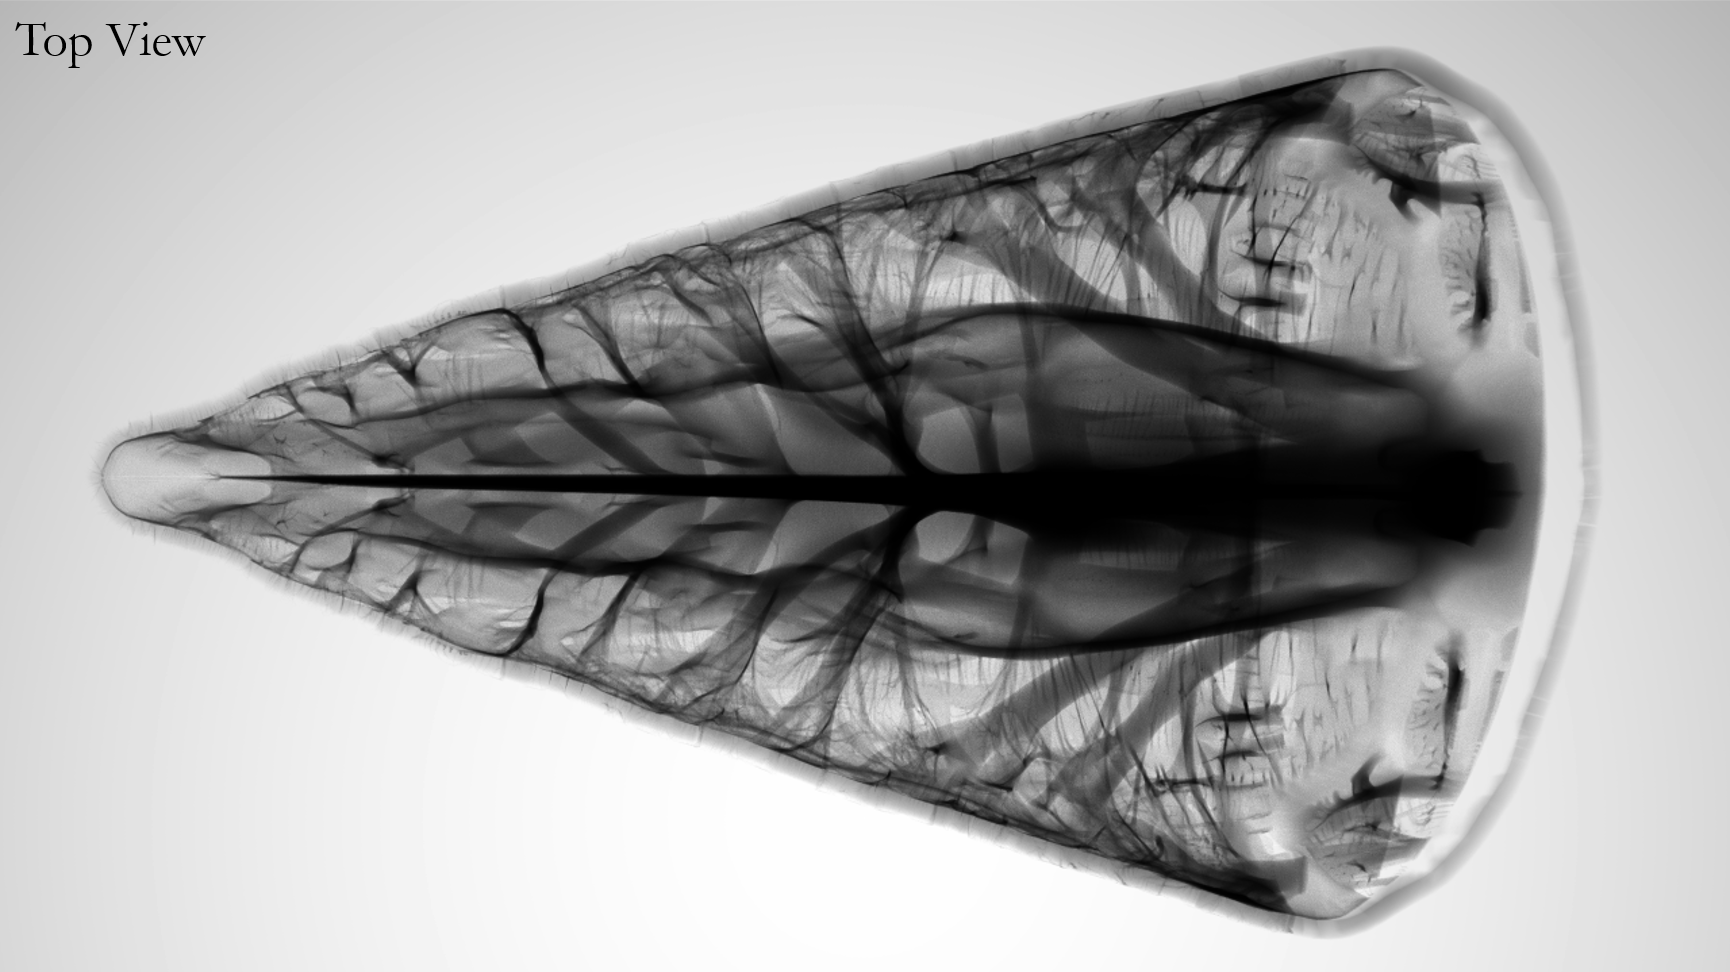
\includegraphics[width=0.39\textwidth]{Beak}
\end{wrapfigure}
The state of the art solvers can only achieve resolution that is an order of magnitude smaller in a single computer.By utilizing AVX instructions on modern CPUs and a novel data structure that uses virtual memory system we achieved optimization of a domain 3000 x 2400 x 1600 with 1.04 billion active voxels on a single computer(Right image)\cite{TopOptimization}.

\textbf{Adaptive Second Order Liquid Simulation.} Using adaptive data structure is an effective way to focus computation resources on visually interesting regions. Traditional adaptive algorithms for fluid simulation always requires the surface of the water to be simulated at the most refined resolution. Such constraint not only is costly due to the requirement of re-creating the simulation grid every frame due to the movement of the fluid surface, 
\begin{wrapfigure}{l}{0.5\textwidth}
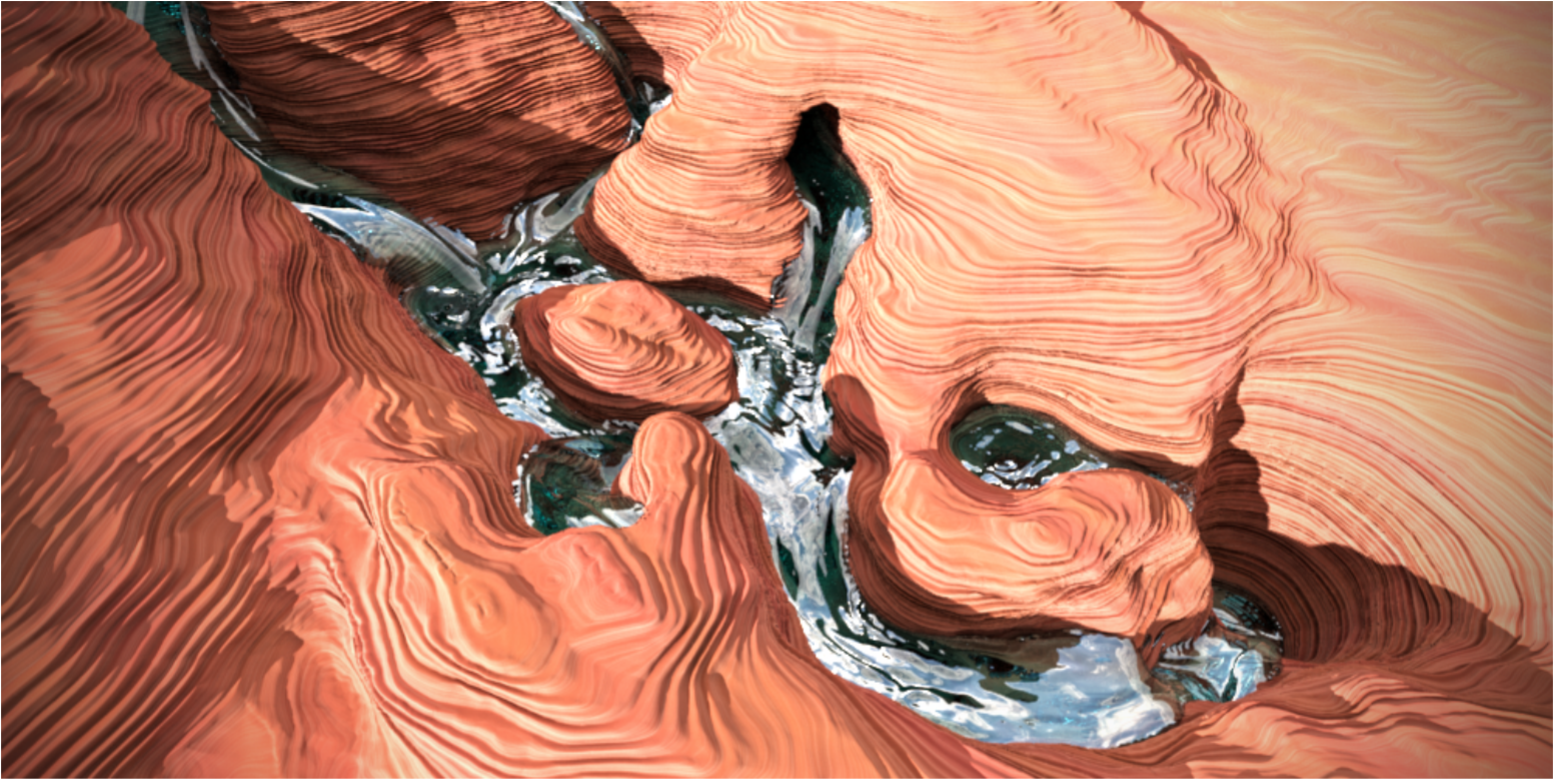
\includegraphics[width=0.49\textwidth]{River}
\end{wrapfigure}
but also preventing the concentration of simulation resolution onto visually interesting regions, for instance where the fluid meets the obstacles or where the steams meet. 
We developed a method that lifts this constraint\cite{Power}. This has enabled the simulation of large water body, with increased resolution along the interface where water and the geometric boundary meet(Left image). 

\textbf{Domain Decomposition Algorithm for Heterogeneous Platform.} Modern GPUs and other accelerators(Xeon Phi for example) are packed with computation FLOPS(floating points operations per second) and memory bandwidth that are close to an order of magnitude higher than a CPU. But the memory capacity are limited. Simulations are memory demanding, and when the simulation demands more memory than the accelerator have, it would be prohibitive to use the accelerator in such a case.
\begin{wrapfigure}{r}{0.4\textwidth}
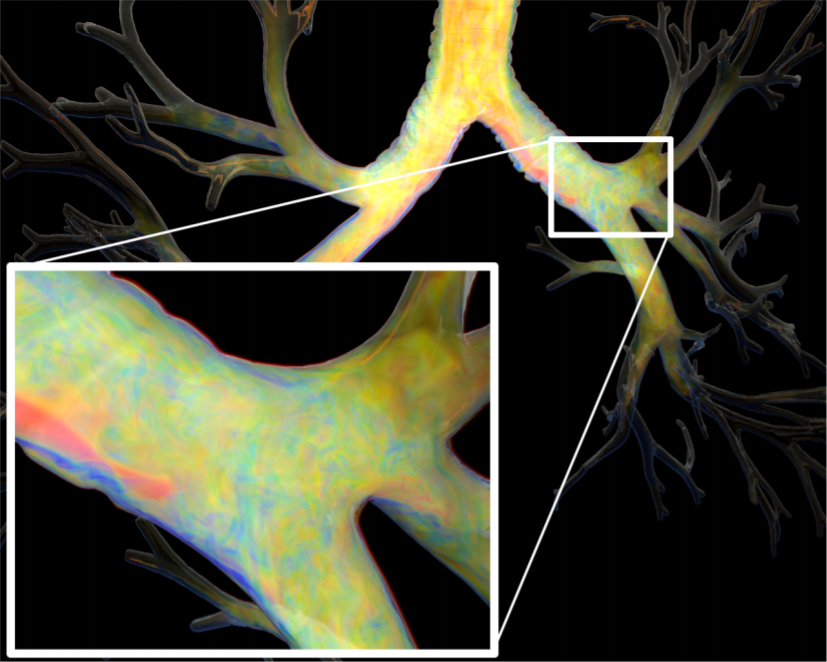
\includegraphics[width=0.39\textwidth]{Bronki}
\end{wrapfigure} 
We developed a Domain Decomposition Method that utilize multiple accelerators for simulating domains that would require more memories than each of them has. By dividing the simulation domain into small pieces that each fits onto a single accelerator, we devised a novel algorithm that utilize the computation capability of each of the accelerators, while minimizing the communication between them over a slow bus. Right image is a simulation of smoke inside a model of the bronchi with 1.8 billion active cells and a grid resolution of $8192 \times 8192 \times 4096$.

\section*{Research interests}

\textbf{Linear Cost Numerical Solvers for Simulation.} Numerical simulations often require solving large sparse linear systems. But conventional sparse solvers have super-linear cost. When venturing into higher resolution, this super-linear cost makes the solve stage dominating the total simulation time. There is a class of solvers named multigrid method that can provide a solution at linear cost for homogeneous problems. But with domains of complex geometry and largely varying materials, the convergence of the algorithm decrease drastically and lost it's linear cost property. I am currently investigating algorithms that can restore the convergence property of the multigrid method even under complex domains.

\textbf{Validation of Simulation for Non-linear Elasticity.} Validation is an important process when acquired a simulation result, for it is the confidence that the result is useful in predicting reality. There are two aspects of validation: First, the validation of the numerical solution converges to the continuous solution under refinement. Second is the validation of the material model in describing the physical material. For materials such as metal or concrete, the linear elastic material model has proven to be effect and accurate. But for soft materials that are still only vary limit understanding in the accuracy of the simulation results. I am interested in developing frameworks for the validation of simulation results for soft materials.

\begin{thebibliography}{99}

\bibitem{TopOptimization}
 H. Liu*, Y. Hu*, B. Zhu, W. Matusik, E. Sifakis. Narrow-Band Topology Optimization on a Sparsely Populated Grid (Submitted and accepted by Proceedings of ACM SIGGRAPH Asia), 2018

\bibitem{Power}
M. Aanjaneya*, M. Gao*, H. Liu, C. Batty, E. Sifakis. Power Diagrams and Sparse Paged Grids for High Resolution Adaptive Liquids, ACM Transactions on Graphics 36:4 (Proceedings of ACM SIGGRAPH), 2017

\bibitem{DD}
H. Liu, N. Mitchell, M. Aanjaneya, E. Sifakis. A scalable Schur-complement fluids solver for heterogeneous compute platforms,  ACM Transactions on Graphics 35:6 (Proceedings of ACM SIGGRAPH Asia), 2016
\end{thebibliography}

\end{document}


